\insertmeeting 
	{Kickoff!} 
	{09/10/22} 
	{Hagerty High School}
	{Jorge, Karissa, Laura, Mohana, Nathan, Robert, Samantha, Tyler, Ritam, Anouska, Jensen}
	{Images/RobotPics/robot.jpg}
	{11:30 - 2:30}
	
\hhscommittee{General}
\noindent\hfil\rule{\textwidth}{.4pt}\hfil
\subsubsection*{Goals}
\begin{itemize}
    \item Watch kickoff
    \item Brainstorm hardware ideas

\end{itemize} 

\noindent\hfil\rule{\textwidth}{.4pt}\hfil

\subsubsection*{Accomplishments}
Today we watched the kickoff with our team. The start of a new season is always exciting and this year is no exception. Our team discussed the possible drivetrains and did some post-reveal planning of hardware and also driving paths around the field. At the moment, what drivetrain we are going to pick is still up in the air. However, we are considering mecanum and car drivetrains. Mecanum would be useful because of the ability to strafe between poles, however, our driver already has extensive practice with the car drive train. The car drive is lighter than mecanum but lacks the maneuverability of mecanum. As for intake designs there are a few ideas floating around among the team. One is to have an arm protruding from the side of the robot that rotates around one axis. 
However, such an arm might be awkward to line up. Another idea was to use a forklift like design which would have a linear slide on a linear slide to reach the heights it needs to. It would push into a cone to pick it up then raise it up to reach the highest goal. However this design has some problems. One is that it would be heavy and likely slow and it would also be fairly complex compared to other opinions. Along the same vein of this idea we had the idea of putting a pivoting arm on a linear slide. This idea would need some kind of 4 bar to work effectively so the cone could be lowered onto the goals. It would also have the same problems as the forklift in being heavy and complex.



\begin{figure}[ht]
\centering
\begin{minipage}[b]{.48\textwidth}
  \centering
  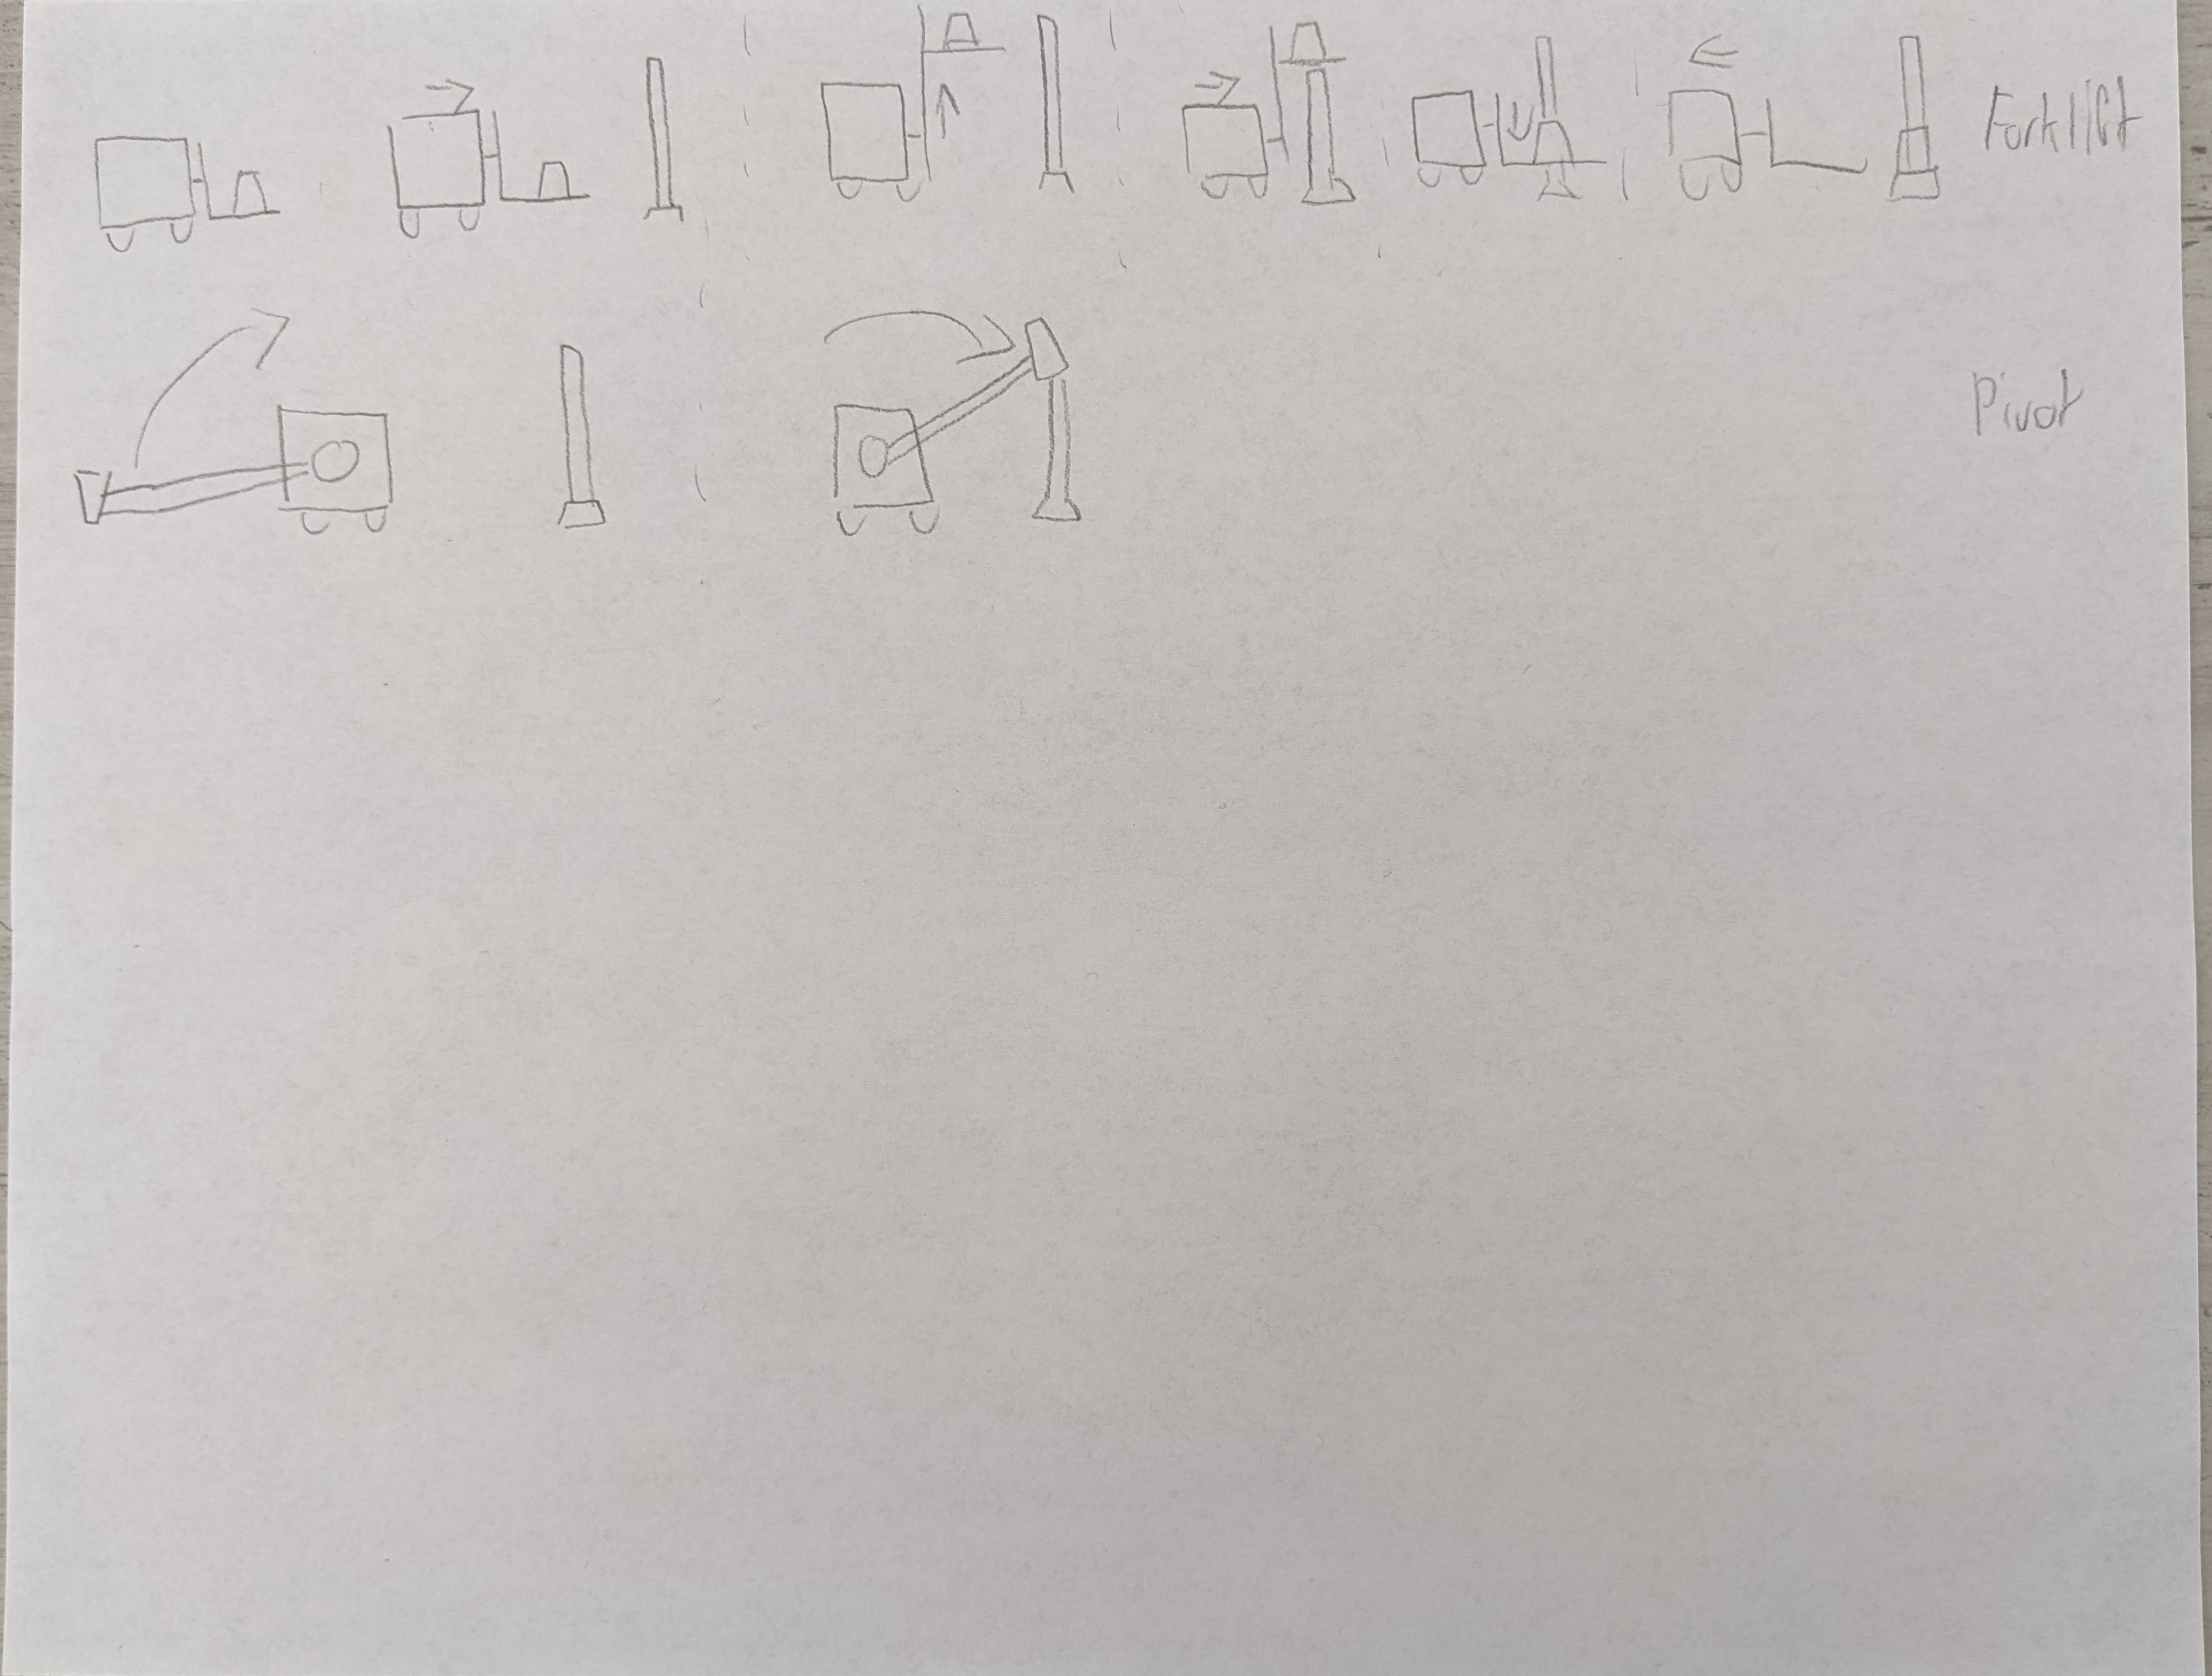
\includegraphics[width=0.95\textwidth]{Meetings/September/09-10-22/09-10-22-Design.jpg}
  \caption{Forklift or Pivot arm?}
  \label{fig:pic1}
\end{minipage}%

\hfill%
\begin{minipage}[b]{.48\textwidth}
  \centering
  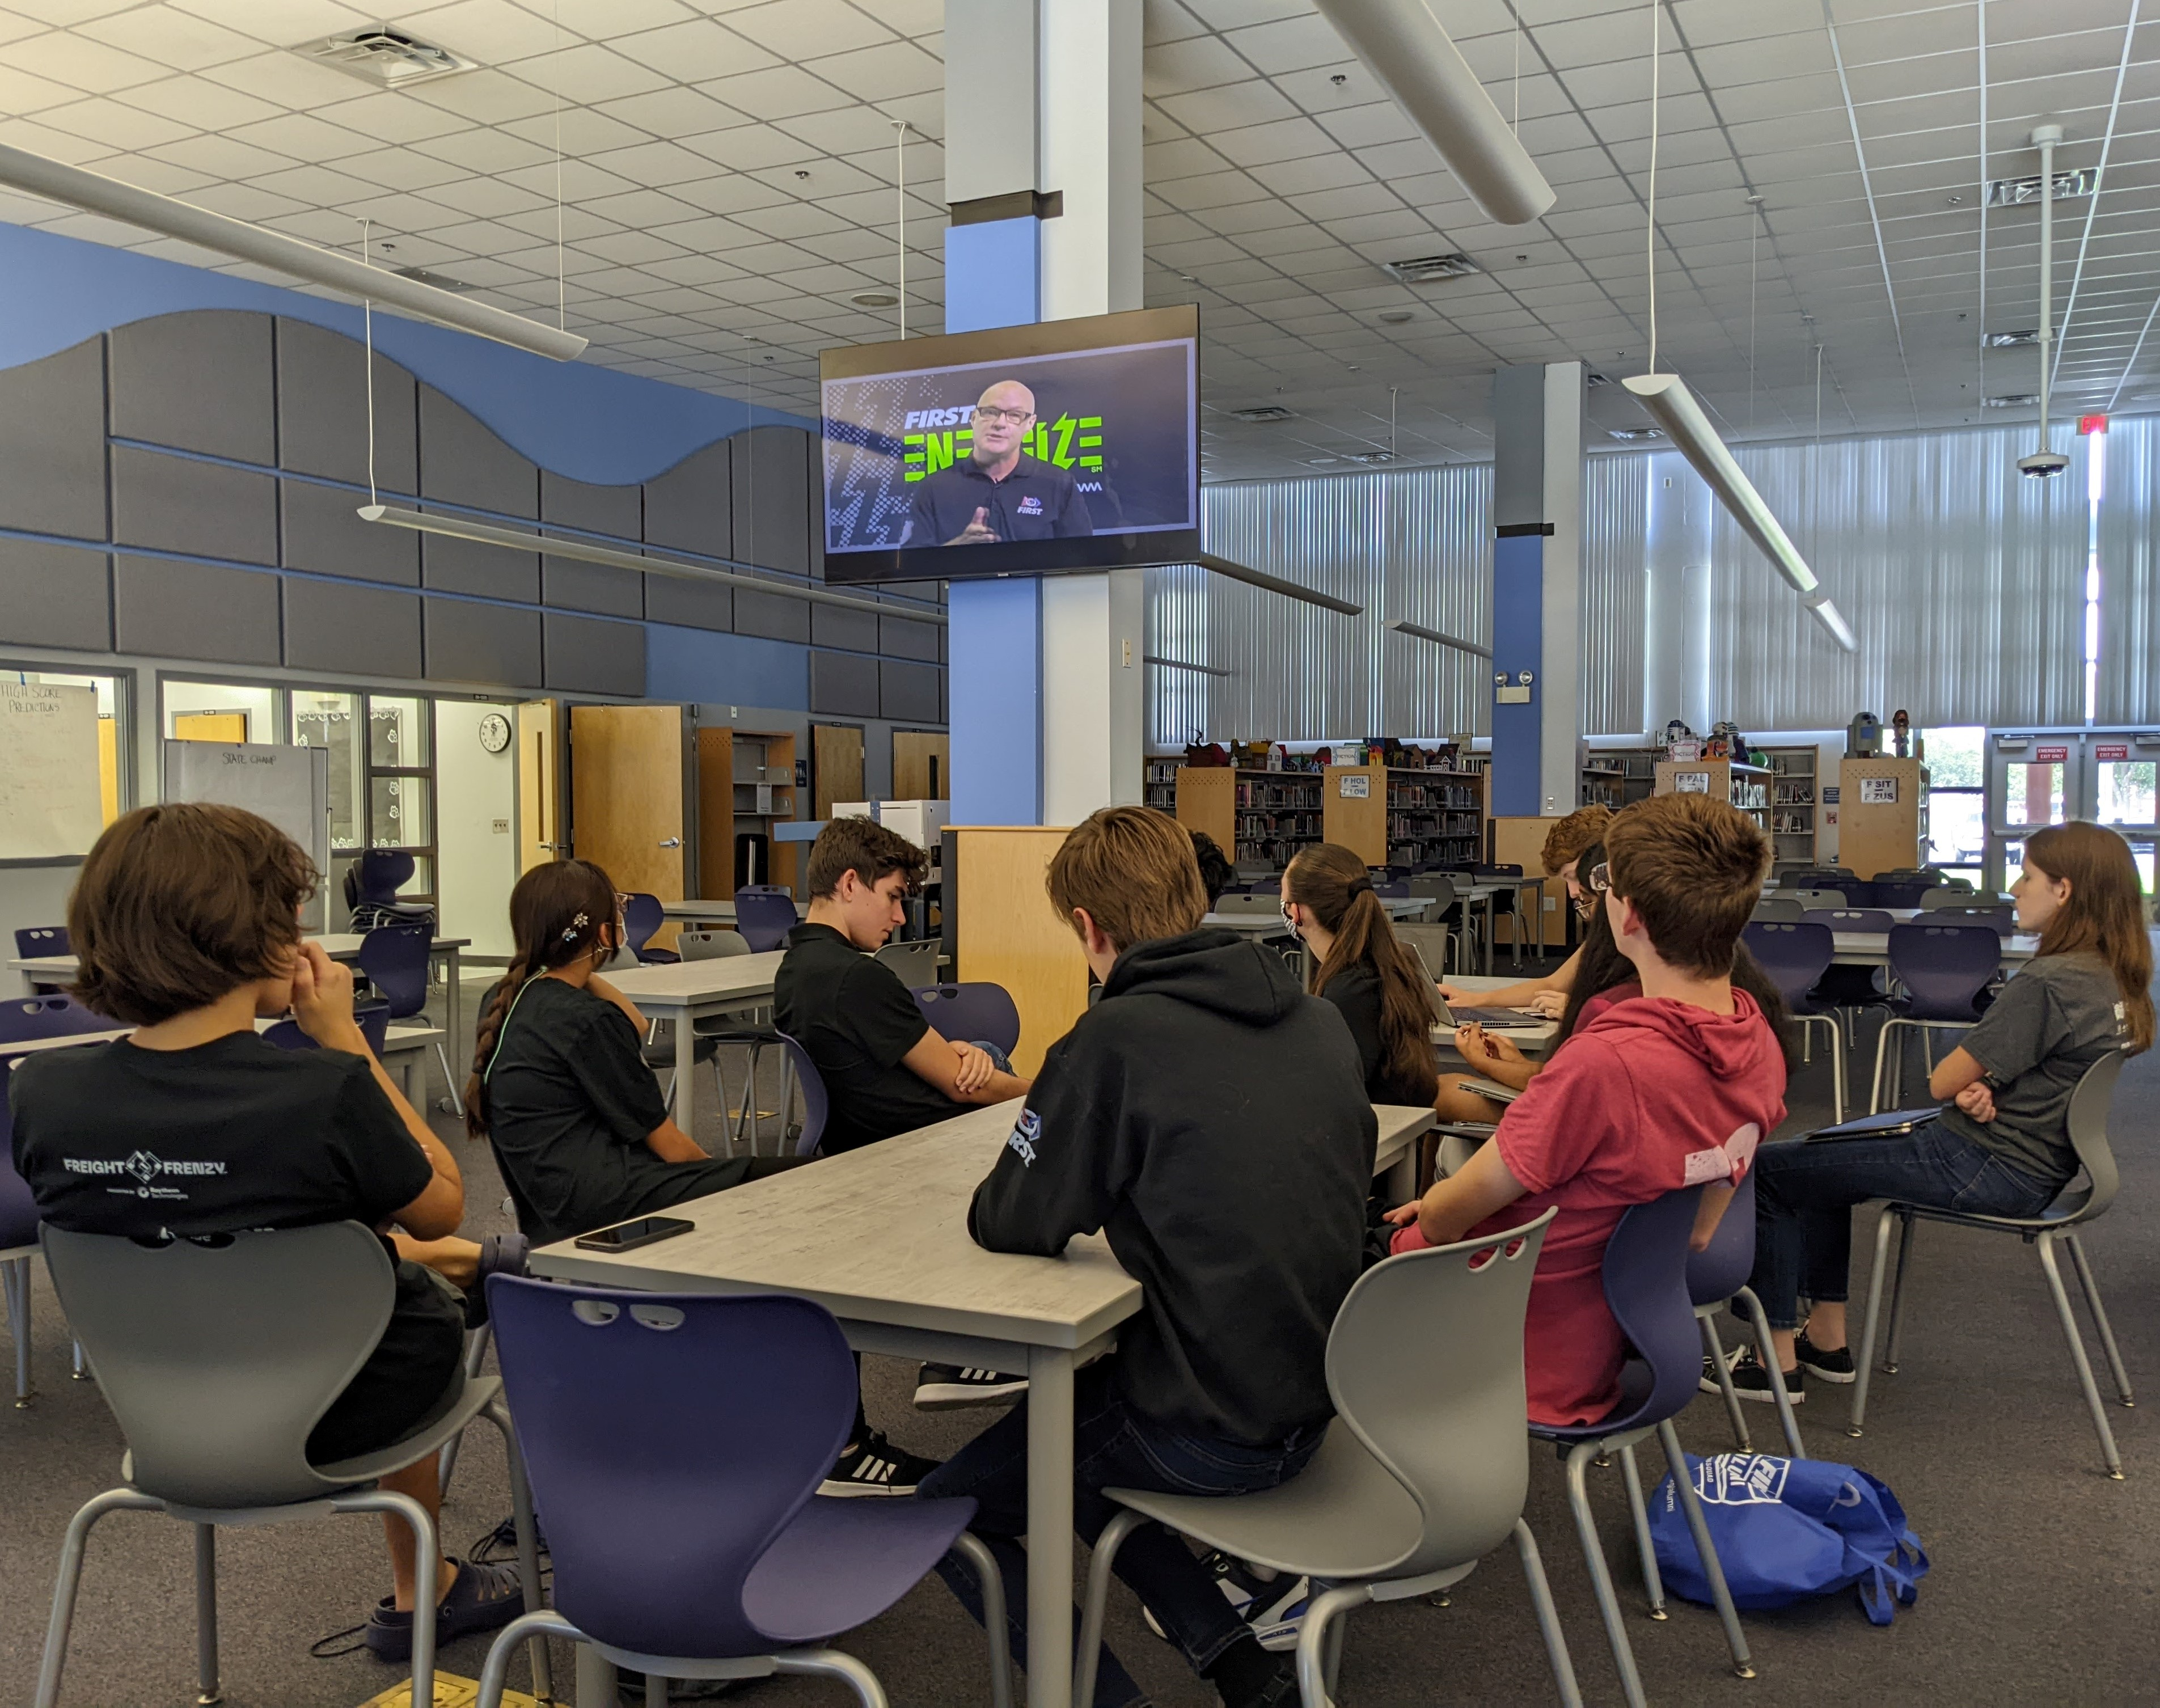
\includegraphics[width=0.95\textwidth]{Meetings/September/09-10-22/09-10-22-Team.jpg}
  \caption{Team at kickoff}
  \label{fig:pic2}
\end{minipage}
\end{figure}

\begin{figure}[htp]
\centering
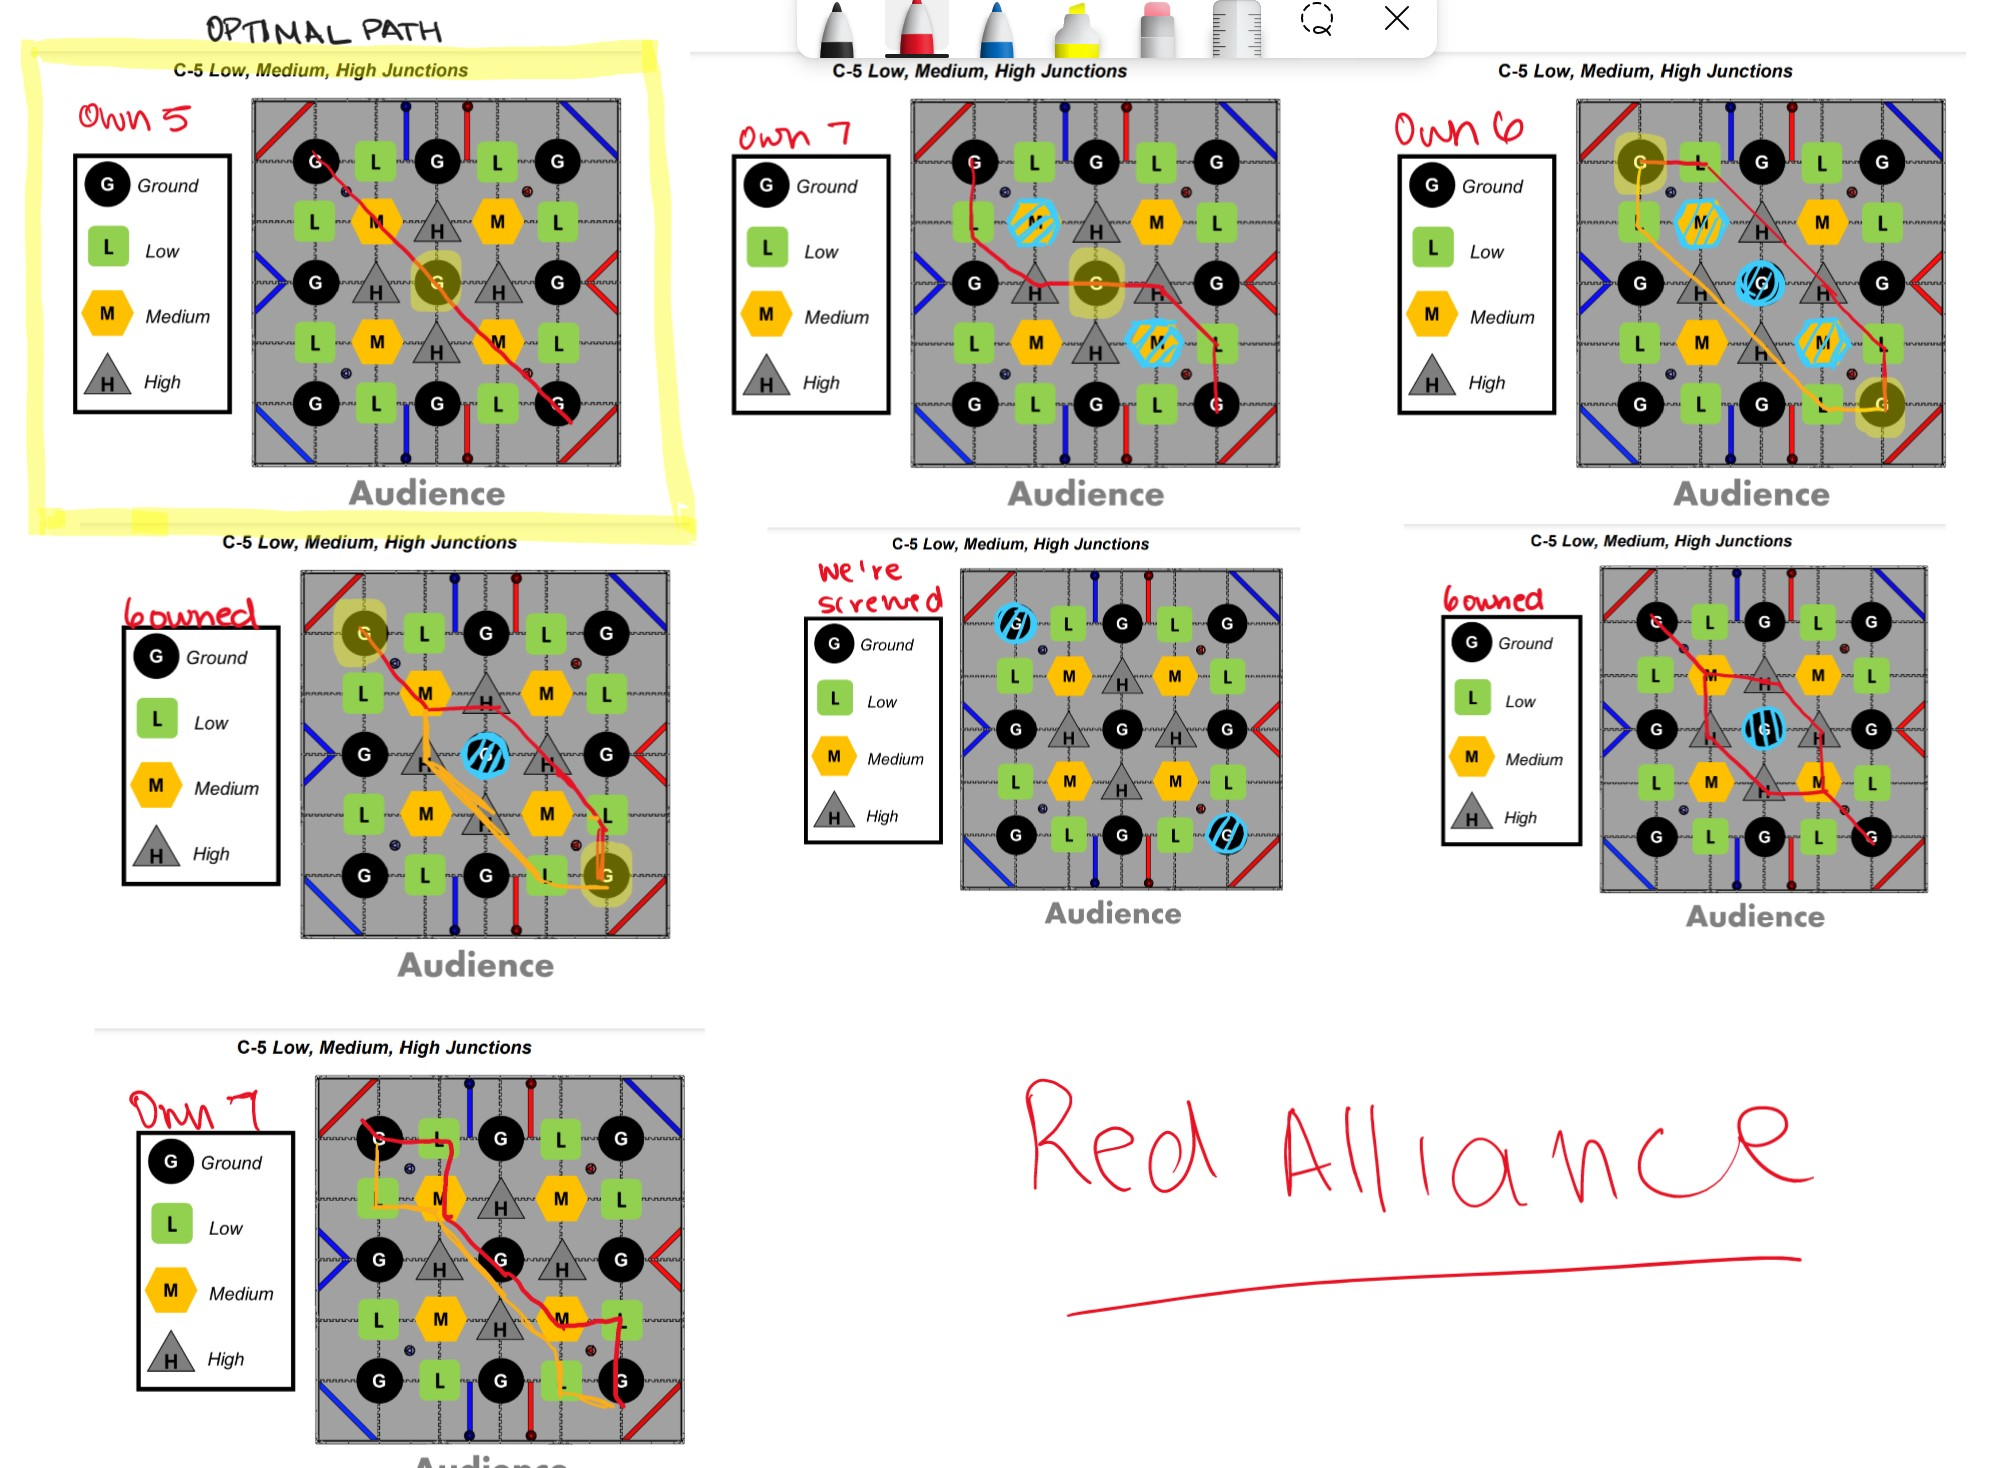
\includegraphics[width=0.95\textwidth, angle=0]{Meetings/September/09-10-22/09-10-22-Paths.jpg}
\caption{Sketch of possible circuit paths on Red Alliance}
\label{fig:pic3}
\end{figure}

\whatsnext{
\begin{itemize}
    \item Propose hardware designs
    \item Think about possible outreach and professionals we can reach out to
    \item Ways to complete a circuit
    
    
\end{itemize} 
}
